

\documentclass[review,authoryear, 12pt]{elsarticle}\usepackage[]{graphicx}\usepackage[]{color}
%% maxwidth is the original width if it is less than linewidth
%% otherwise use linewidth (to make sure the graphics do not exceed the margin)
\makeatletter
\def\maxwidth{ %
  \ifdim\Gin@nat@width>\linewidth
    \linewidth
  \else
    \Gin@nat@width
  \fi
}
\makeatother

\definecolor{fgcolor}{rgb}{0.345, 0.345, 0.345}
\newcommand{\hlnum}[1]{\textcolor[rgb]{0.686,0.059,0.569}{#1}}%
\newcommand{\hlstr}[1]{\textcolor[rgb]{0.192,0.494,0.8}{#1}}%
\newcommand{\hlcom}[1]{\textcolor[rgb]{0.678,0.584,0.686}{\textit{#1}}}%
\newcommand{\hlopt}[1]{\textcolor[rgb]{0,0,0}{#1}}%
\newcommand{\hlstd}[1]{\textcolor[rgb]{0.345,0.345,0.345}{#1}}%
\newcommand{\hlkwa}[1]{\textcolor[rgb]{0.161,0.373,0.58}{\textbf{#1}}}%
\newcommand{\hlkwb}[1]{\textcolor[rgb]{0.69,0.353,0.396}{#1}}%
\newcommand{\hlkwc}[1]{\textcolor[rgb]{0.333,0.667,0.333}{#1}}%
\newcommand{\hlkwd}[1]{\textcolor[rgb]{0.737,0.353,0.396}{\textbf{#1}}}%

\usepackage{framed}
\makeatletter
\newenvironment{kframe}{%
 \def\at@end@of@kframe{}%
 \ifinner\ifhmode%
  \def\at@end@of@kframe{\end{minipage}}%
  \begin{minipage}{\columnwidth}%
 \fi\fi%
 \def\FrameCommand##1{\hskip\@totalleftmargin \hskip-\fboxsep
 \colorbox{shadecolor}{##1}\hskip-\fboxsep
     % There is no \\@totalrightmargin, so:
     \hskip-\linewidth \hskip-\@totalleftmargin \hskip\columnwidth}%
 \MakeFramed {\advance\hsize-\width
   \@totalleftmargin\z@ \linewidth\hsize
   \@setminipage}}%
 {\par\unskip\endMakeFramed%
 \at@end@of@kframe}
\makeatother

\definecolor{shadecolor}{rgb}{.97, .97, .97}
\definecolor{messagecolor}{rgb}{0, 0, 0}
\definecolor{warningcolor}{rgb}{1, 0, 1}
\definecolor{errorcolor}{rgb}{1, 0, 0}
\newenvironment{knitrout}{}{} % an empty environment to be redefined in TeX

\usepackage{alltt}

\usepackage{graphicx}
\usepackage{caption}
\usepackage{subcaption}
\usepackage{filecontents}
\usepackage{comment}
\usepackage{amssymb}
\usepackage{amsthm}
\usepackage{amsmath,bm}
\usepackage[utf8]{inputenc}
\usepackage{rotating}
\usepackage{natbib}
\usepackage{gensymb}
%\journal{Geothermics Journal}



\IfFileExists{upquote.sty}{\usepackage{upquote}}{}
\begin{document}
%\nocite{*}
\begin{frontmatter}

%\author{Esmail Ansari}
%\ead{eansar2@lsu.edu}
%\author{Richard Hughes}

\title{Statistical Analysis of the Gulf Coast Geothermal Reservoirs}
%\address{Louisiana State University}

\begin{abstract}

Important parameters of the Gulf Coast geothermal reservoirs are investigated. They are: permeability, porosity, average reservoir temperature, thickness, length (i.e. area\textsuperscript{0.5}), temperature gradient of the earth, reservoir dip angle, injection temperature and well flow rate. The data, used to create the range and distribution of the parameters, come from previous reports on the subject. These data were transformed using appropriate methods and a distribution is fit to the transformed data. An approach for calculating the reservoir dip angle is presented which requires bootstrapping the temperature gradient in the area. This paper provides ground for experimental design and scaling analysis studies. 

\end{abstract}


\end{frontmatter}




\section{Available data and limitations}
The geothermal data used in this study is based on the reports published by    \citet{bassiouni1980evaluation} and \citet{john1998gulf}. The sources contain the data collected in the Wells-of-Opportunity  and Design Wells program, repectively. 
 
 
In the Wells-of-Opportunity program (1975), the wells were selected from the conventional dry holes based on necessary criteria for potentially productive geopressured geothermal aquifers. The program was designed to quickly provide information on the physical and petrophysical characteristics of a large number of reservoirs from a diverse geographic and geologic area whitough great expense. Such a program has the limitation of not locating the well in structurally favorable locations and pressure transient tests would not provide the information on the complete reservoir limits.  The program finally ranks the fifteen most promising geopressure geothermal prospects in the Louisiana out of sixty-three prospects. These fifteen wells exist in the dataset labeled as Source 1; all of which have reservoir volume and depth information. Only for the best five wells, permeability, porosity and temperature data are available \citep{bassiouni1980evaluation}. 

The Design Well program was conducted between 1979-1990 to provide long term  comprehensive information from wells located at optimum reservoir points and designed to produce geopresured brines at high rates from geologically favorable areas (Figure \ref{Fig:map_perm}). The data contains temperature, depth, porosity, permeability, flow rate and other unused data (see \texttt{.csv} file) for all the seventeen wells reported for this program, three of which are located in the state of texas \citep{john1998gulf}.

Having said all these limitations, we assume that the data is collected randomly and compare the two data sources using t test and ANOVA for any inconsistency. We further prepare a dynamic document, any new information can go into the accompanied \texttt{.csv} file and the analysis can be regenerated (Table \ref{Tab:DataSummary}). 


\begin{knitrout}
\definecolor{shadecolor}{rgb}{0.969, 0.969, 0.969}\color{fgcolor}\begin{figure}[]

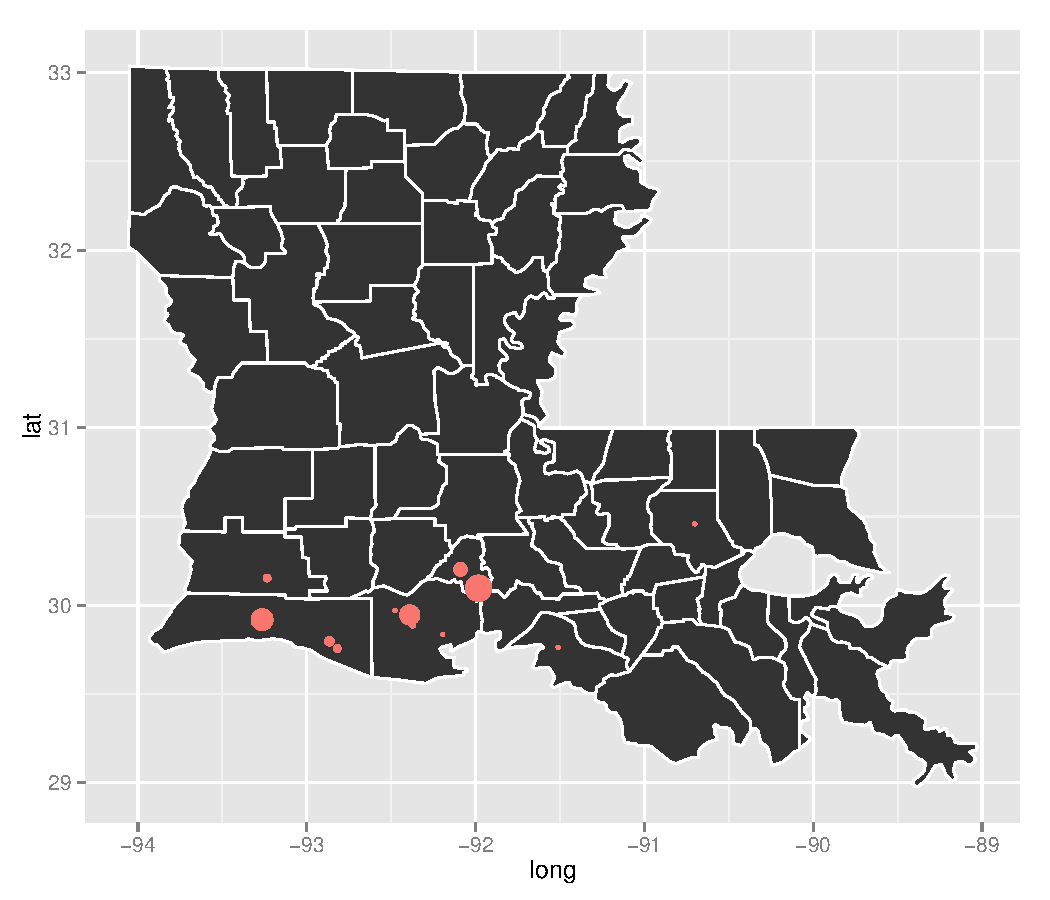
\includegraphics[width=\maxwidth]{figure/map_perm} \caption[Location of only source 2 geothermal reservoirs]{Location of only source 2 geothermal reservoirs. There are also three reservoirs from the Texas which are not shown here. Red dots shows permeability which varies between 7 and 500 md.\label{Fig:map_perm}}
\end{figure}


\end{knitrout}



% latex table generated in R 3.1.1 by xtable 1.7-3 package
% Wed Aug 06 14:17:30 2014
\begin{table}[ht]
\centering
\begin{tabular}{rrrrrr}
  \hline
 & permeability.mD & porosity & temperature.C & thickness.m & length.m \\ 
  \hline
Min. & 7.00 & 12.00 & 100.00 & 10.00 & 10200.00 \\ 
  1st Qu. & 21.00 & 18.00 & 125.00 & 83.00 & 11300.00 \\ 
  Median & 85.00 & 22.00 & 150.00 & 114.00 & 11800.00 \\ 
  Mean & 130.00 & 21.00 & 150.00 & 103.00 & 12200.00 \\ 
  3rd Qu. & 200.00 & 26.00 & 175.00 & 137.00 & 12500.00 \\ 
  Max. & 500.00 & 29.00 & 200.00 & 160.00 & 15800.00 \\ 
   \hline
\end{tabular}
\caption{Summary of the available data} 
\label{Tab:DataSummary}
\end{table}




We do a t test to compare permeability, porosity and temperature that come from these two data sources. The result of the t test on these parameters are summarized in Table \ref{Tab:t_test}. 


% latex table generated in R 3.1.1 by xtable 1.7-3 package
% Wed Aug 06 14:17:30 2014
\begin{table}[ht]
\centering
\begin{tabular}{rrrr}
  \hline
 & df & t & p value \\ 
  \hline
Permeability & 10.74 & -0.62 & 0.55 \\ 
  Porosity & 5.13 & -1.11 & 0.31 \\ 
  Temperature & 11.54 & -2.46 & 0.03 \\ 
   \hline
\end{tabular}
\caption{Summary of the t test for permeability, porosity and temperature. Null hypothesis is rejected for permeability and porosity showing consistency in the reports.} 
\label{Tab:t_test}
\end{table}



The true difference in the permeability and porosity mean is equal to zero which indicates that the data that come from the two sources are consistentassuming normality for their underlying theoretical distribution. The t test for the temperature does not reject the null hypothesis indicating that the temperature mean of the groups are different. Nevertheless, this result can be a type two error because the investigation depth of the reports are different. A  two way ANOVA is more appropriate for making final conclusion about temperature.  

% latex table generated in R 3.1.1 by xtable 1.7-3 package
% Wed Aug 06 14:17:30 2014
\begin{table}[ht]
\centering
\begin{tabular}{lrrrrr}
  \hline
 & Df & Sum Sq & Mean Sq & F value & Pr($>$F) \\ 
  \hline
Depth        & 1 & 5185.29 & 5185.29 & 51.83 & 0.0000 \\ 
  Source       & 1 & 146.12 & 146.12 & 1.46 & 0.2444 \\ 
  Depth:Source & 1 & 111.92 & 111.92 & 1.12 & 0.3059 \\ 
  Residuals    & 16 & 1600.56 & 100.04 &  &  \\ 
   \hline
\end{tabular}
\caption{Summary of the two way ANOVA on the temperature. The difference in the temperature is caused by the depth.} 
\label{Tab:temp_anova}
\end{table}


The two way ANOVA test for temperature is summarized in Table \ref{Tab:temp_anova}. The effect of having different temperature mean is soley due to the depth and not the source confirming the consistency between the reports. Rejecting the null hypothesis for permeability, porosity and temperature also provides some preliminary basis to claim that the hot saline aquifers of the Louisiana have gone through similar depositional environment and diagenetic history.


\section{Permeability}
The geological processes that create permeability in reservoir rocks appear to leave permeability distributed around the geometric mean (log normal distribution). The permeability is available for most of the wells (Figure \ref{Fig:PermDotChart}). A normal distribution is fit to the logarithm of permeability using \texttt{fitdistrplus} package (Figure \ref{Fig:perm_fit}, Table \ref{Tab:Permfit}).


\begin{knitrout}
\definecolor{shadecolor}{rgb}{0.969, 0.969, 0.969}\color{fgcolor}\begin{figure}[]

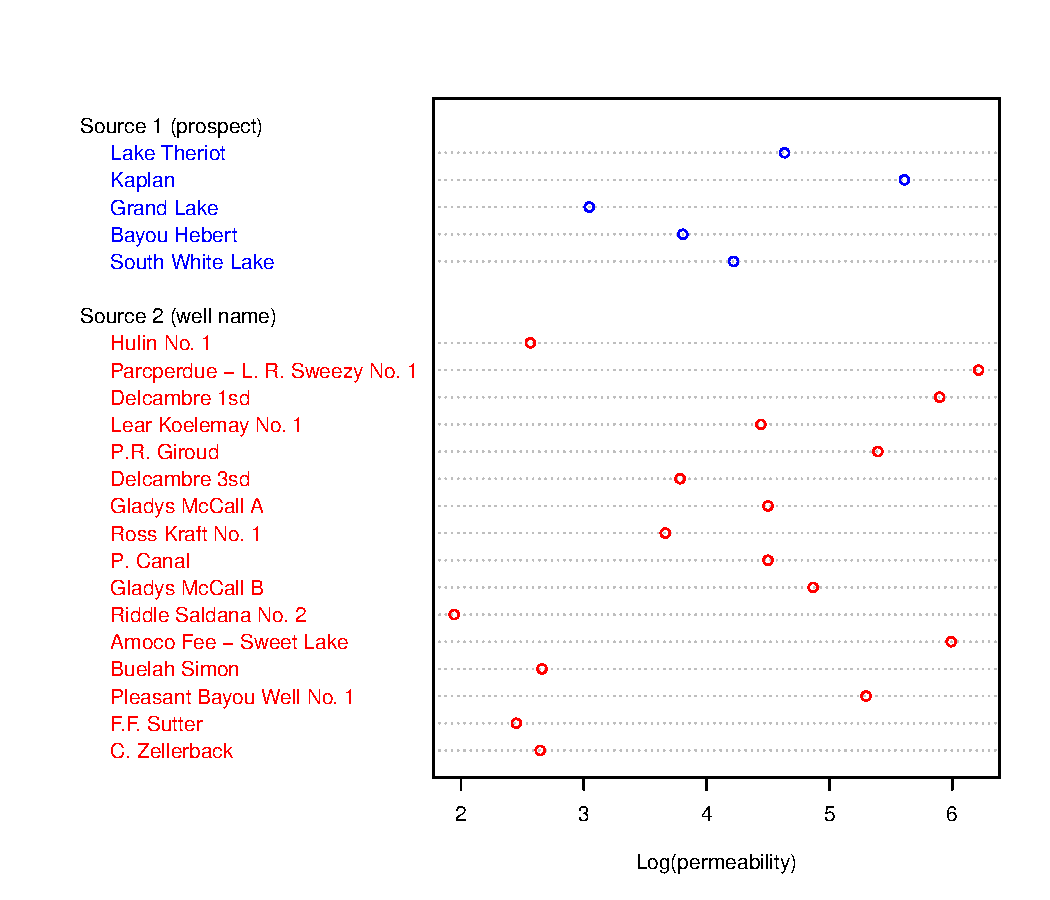
\includegraphics[width=\maxwidth]{figure/PermDotChart} \caption[Log of the permeability sorted by ascending porosity within groups]{Log of the permeability sorted by ascending porosity within groups. Because the data come from different formations and fields, no correlation between porosity and permeability is observed.  . Some of the wells may have missing data which is clear from the \texttt{.csv} file.\label{Fig:PermDotChart}}
\end{figure}


\end{knitrout}


\begin{knitrout}
\definecolor{shadecolor}{rgb}{0.969, 0.969, 0.969}\color{fgcolor}\begin{figure}[]

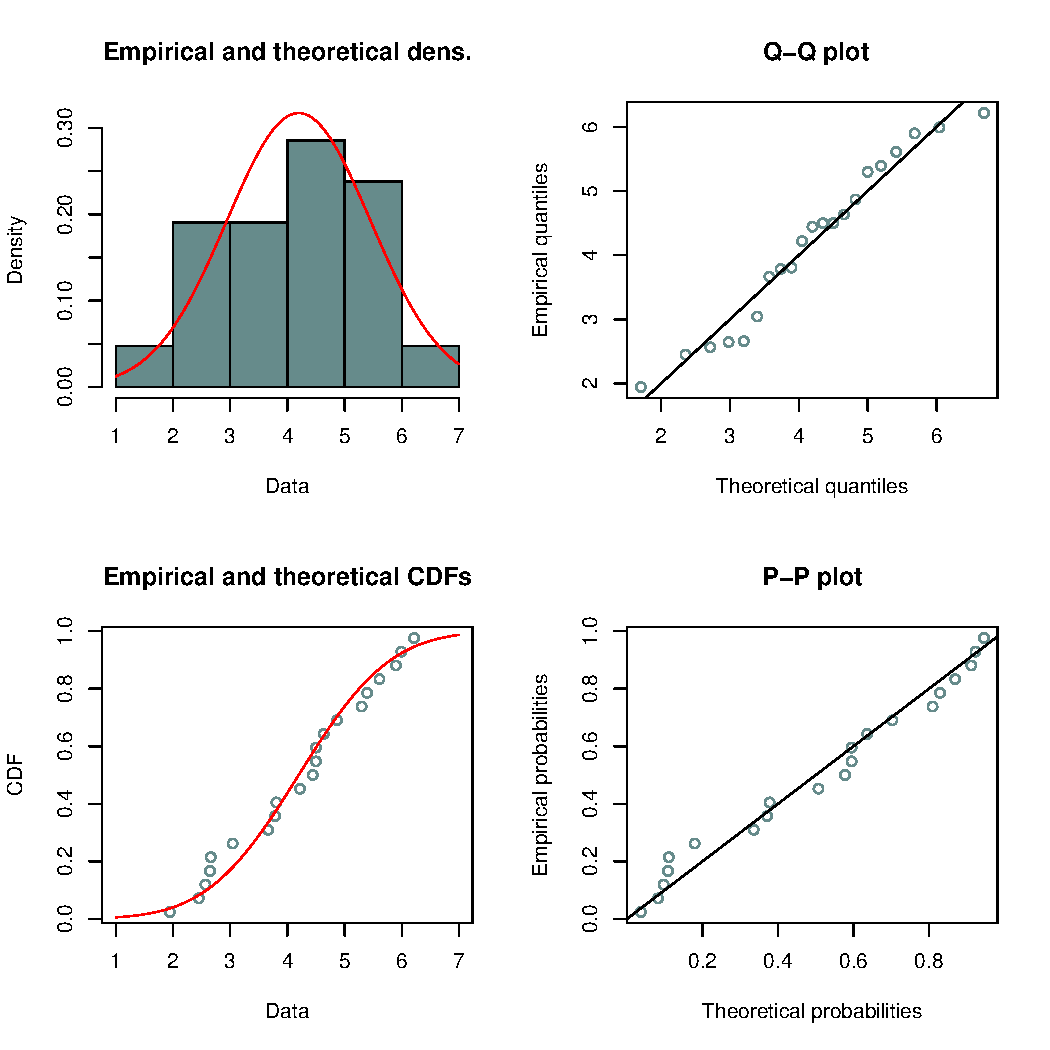
\includegraphics[width=\maxwidth]{figure/perm_fit} \caption[Fitting a normal distribution to the logarithm of permeability]{Fitting a normal distribution to the logarithm of permeability.\label{Fig:perm_fit}}
\end{figure}


\end{knitrout}


% latex table generated in R 3.1.1 by xtable 1.7-3 package
% Wed Aug 06 14:17:31 2014
\begin{table}[ht]
\centering
\begin{tabular}{rr}
  \hline
 & permeability.mD \\ 
  \hline
mean & 4.20 \\ 
  sd & 1.26 \\ 
   \hline
\end{tabular}
\caption{{Summary of the normal fit to the logarithm of permeability}} 
\label{Tab:Permfit}
\end{table}


\pagebreak


\section{Porosity, thickness, length and temperature}
The main underlying assumptions is that the sum of the geological processes that has created porosity, thickness, length and temperature, has left them having a normal distribution. The data (Figure \ref{Fig:histplots}) were transformed using a Box-Cox transform (Figure \ref{Fig:BoxCoxhistplots}) and a Gaussian distribution is then fitted on them (Figure \ref{Fig:poro_BoxCox_fit}). Distribution fitting results are summarized in Table \ref{Tab:poro_etc_fit}.

%-------------------------------------------------
%                    Porosity
%-------------------------------------------------



%-------------------------------------------------------
%                    Average reservoir temperature
%--------------------------------------------------------






%-----------------------------------------------
%                       Thicknesss 
%-----------------------------------------------





%-----------------------------------------------
%                          Length
%-----------------------------------------------



\begin{knitrout}
\definecolor{shadecolor}{rgb}{0.969, 0.969, 0.969}\color{fgcolor}\begin{figure}[]

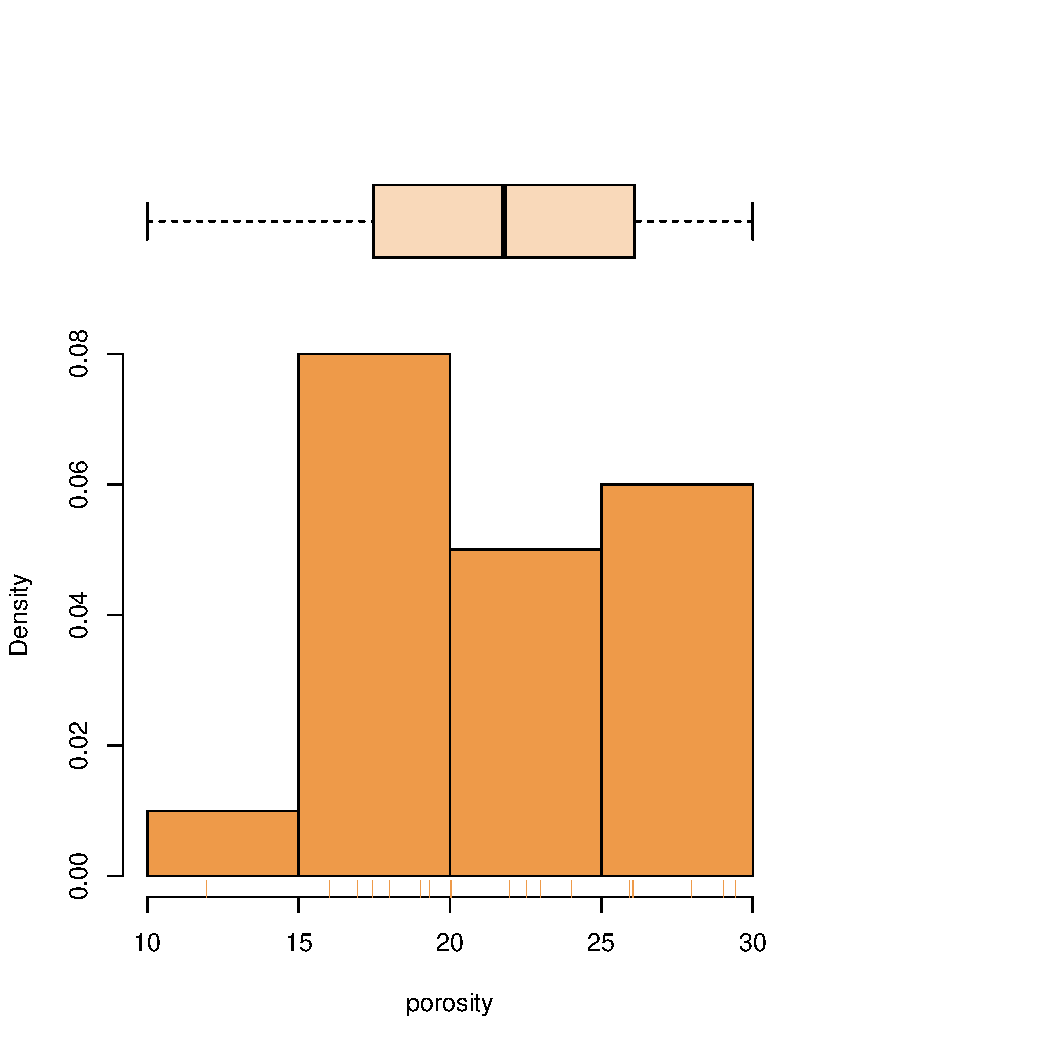
\includegraphics[width=7cm,height=7cm]{figure/histplots1} 
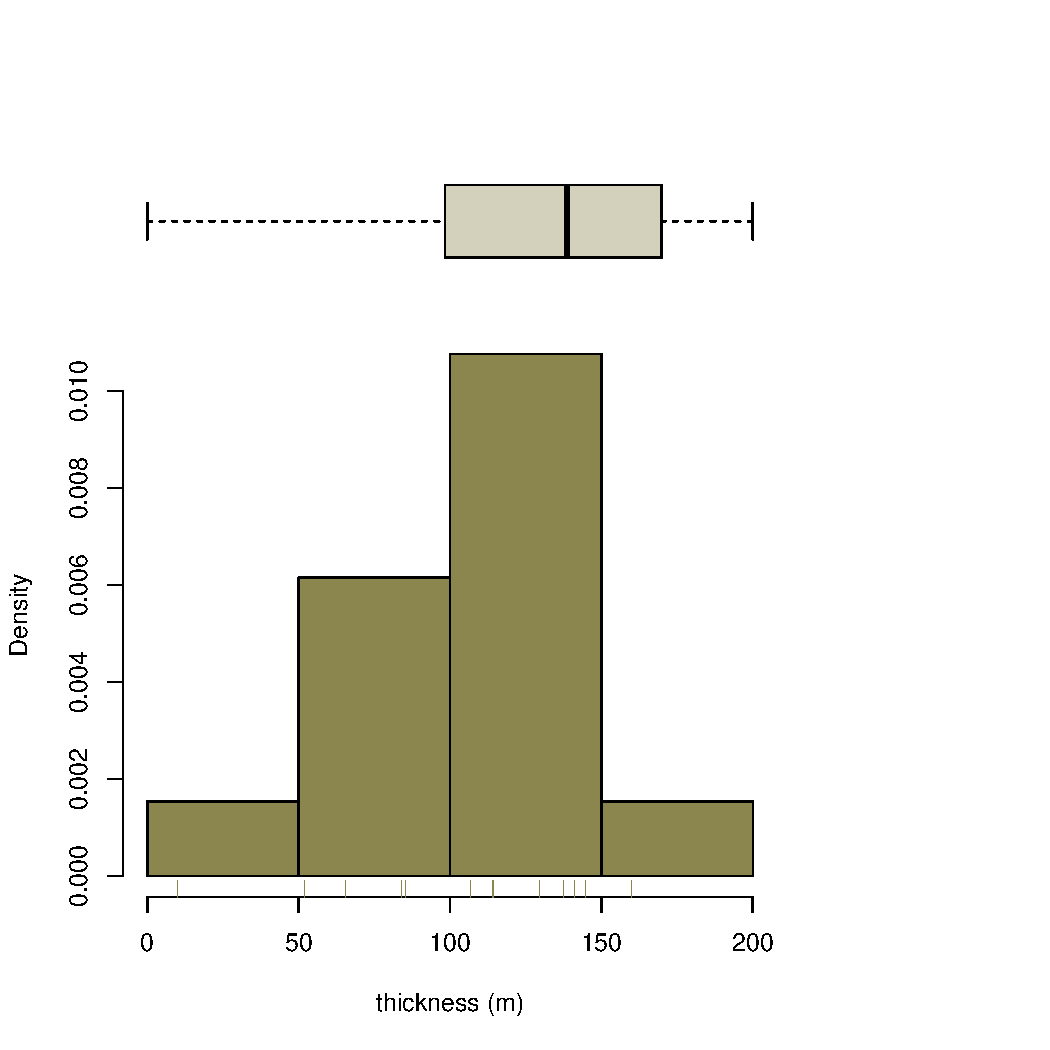
\includegraphics[width=7cm,height=7cm]{figure/histplots2} 
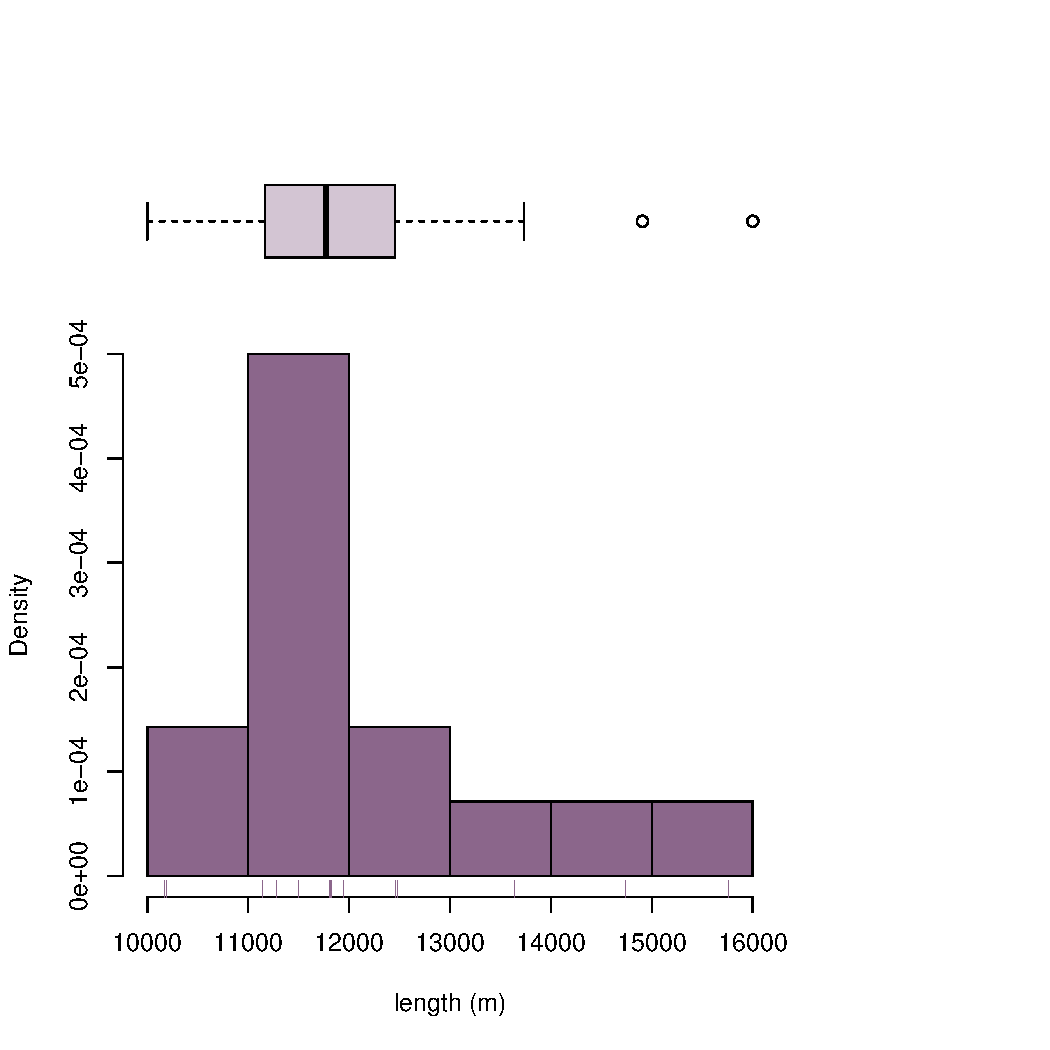
\includegraphics[width=7cm,height=7cm]{figure/histplots3} 
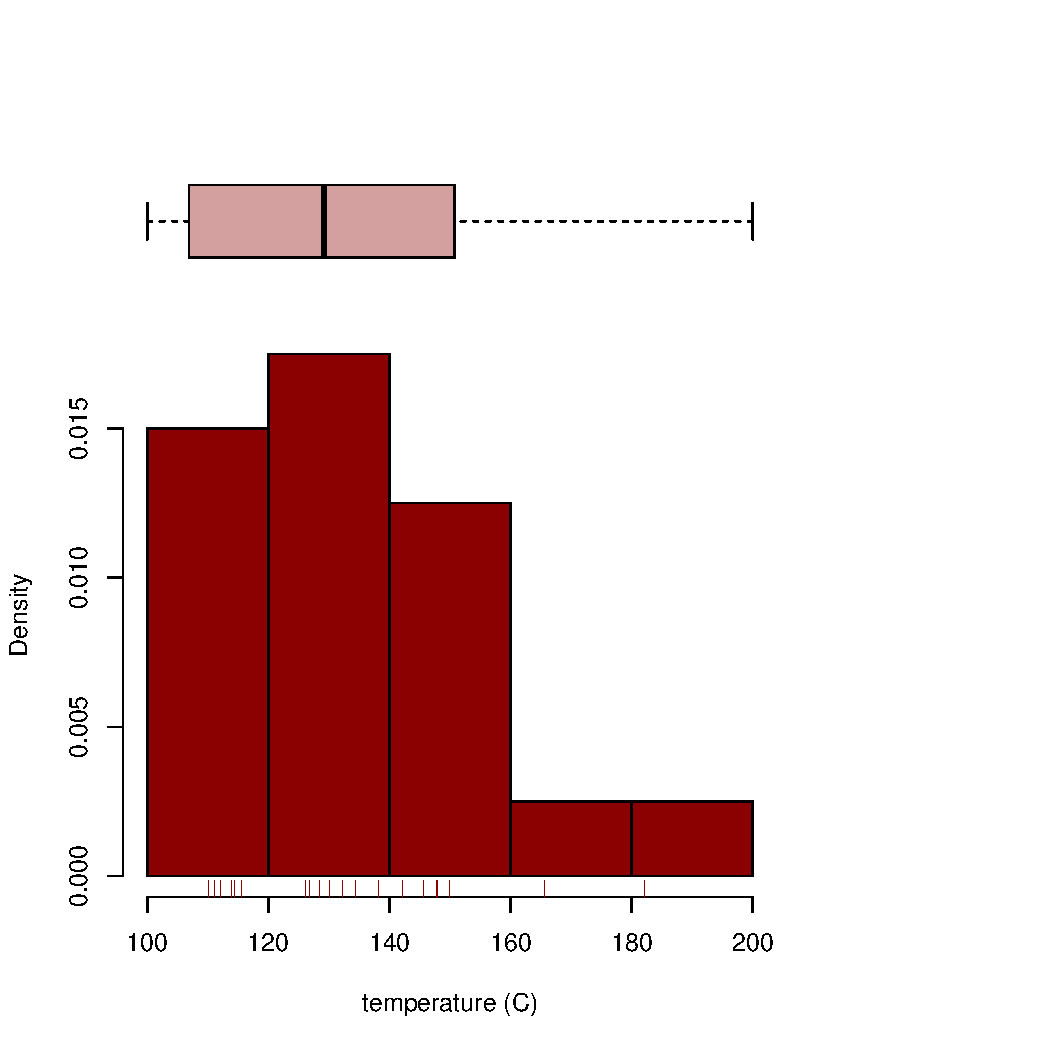
\includegraphics[width=7cm,height=7cm]{figure/histplots4} \caption[Parameter distributions before transformation]{Parameter distributions before transformation. Data values are shown below the historgram as tiny lines and the box plot shows the quantiles of each parameter. The most likely value for the reservoir thickness and length lies between 100-150 m and 11000-12000 m respectively. The most likely value for the porosity and temperature are between 15-20 and 120-140 \degree C, respectively.\label{Fig:histplots}}
\end{figure}


\end{knitrout}


\begin{knitrout}
\definecolor{shadecolor}{rgb}{0.969, 0.969, 0.969}\color{fgcolor}\begin{figure}[]

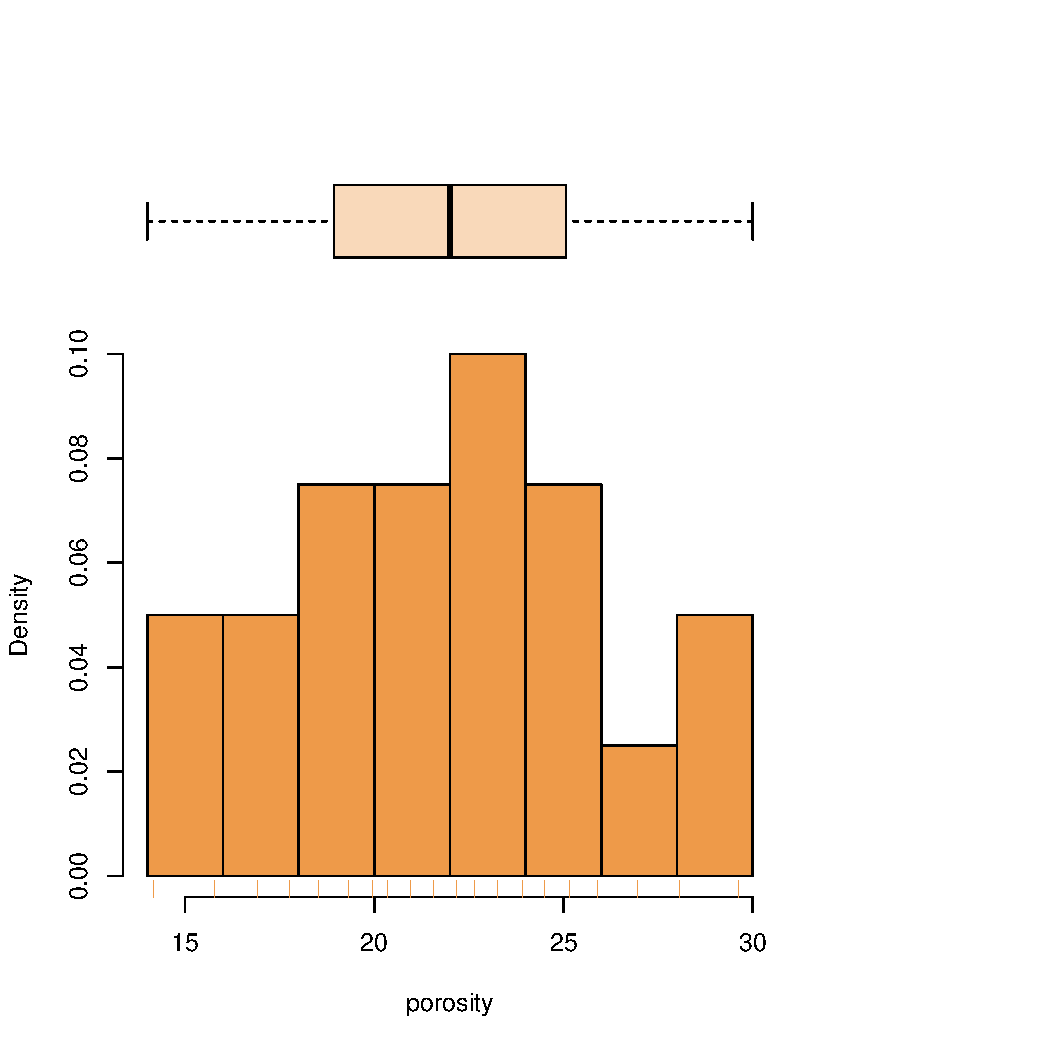
\includegraphics[width=7cm,height=7cm]{figure/BoxCoxhistplots1} 
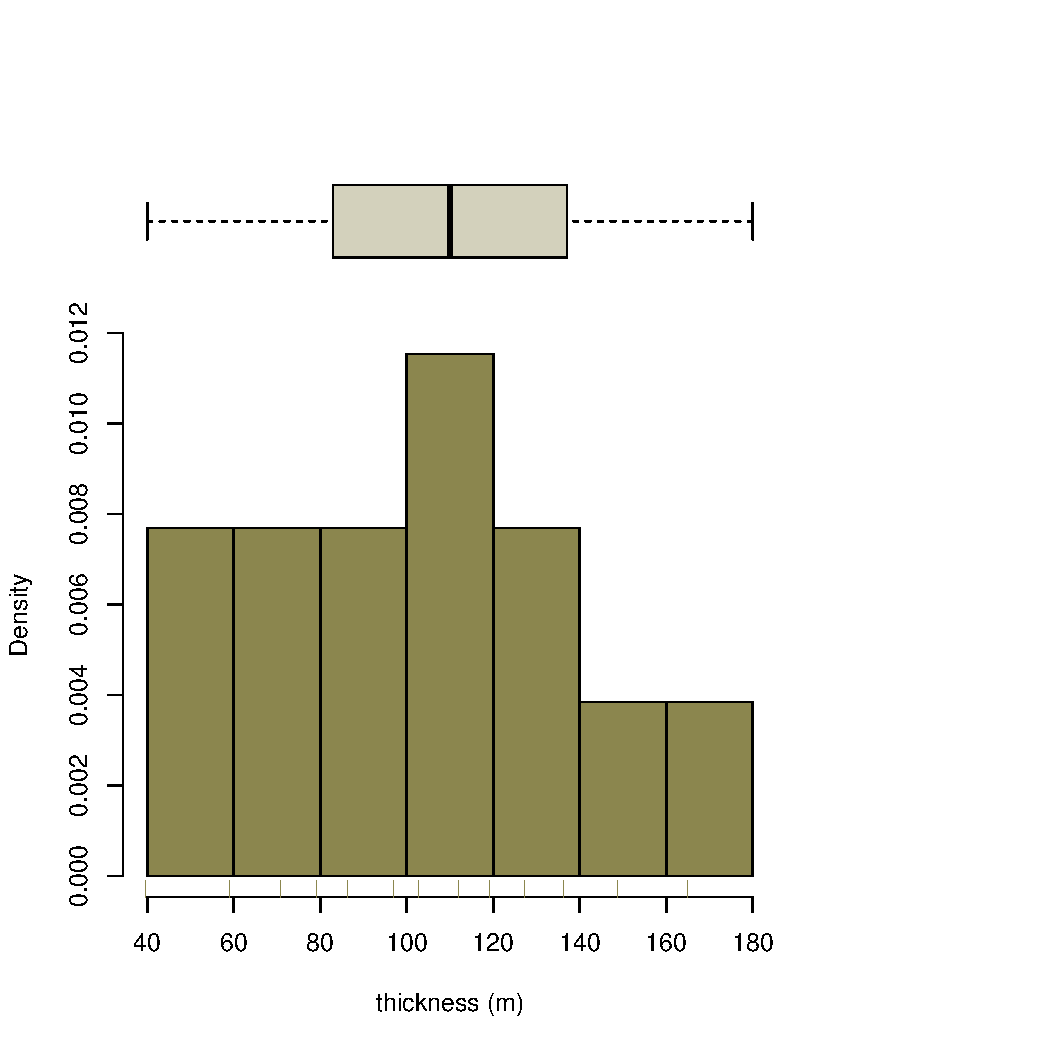
\includegraphics[width=7cm,height=7cm]{figure/BoxCoxhistplots2} 
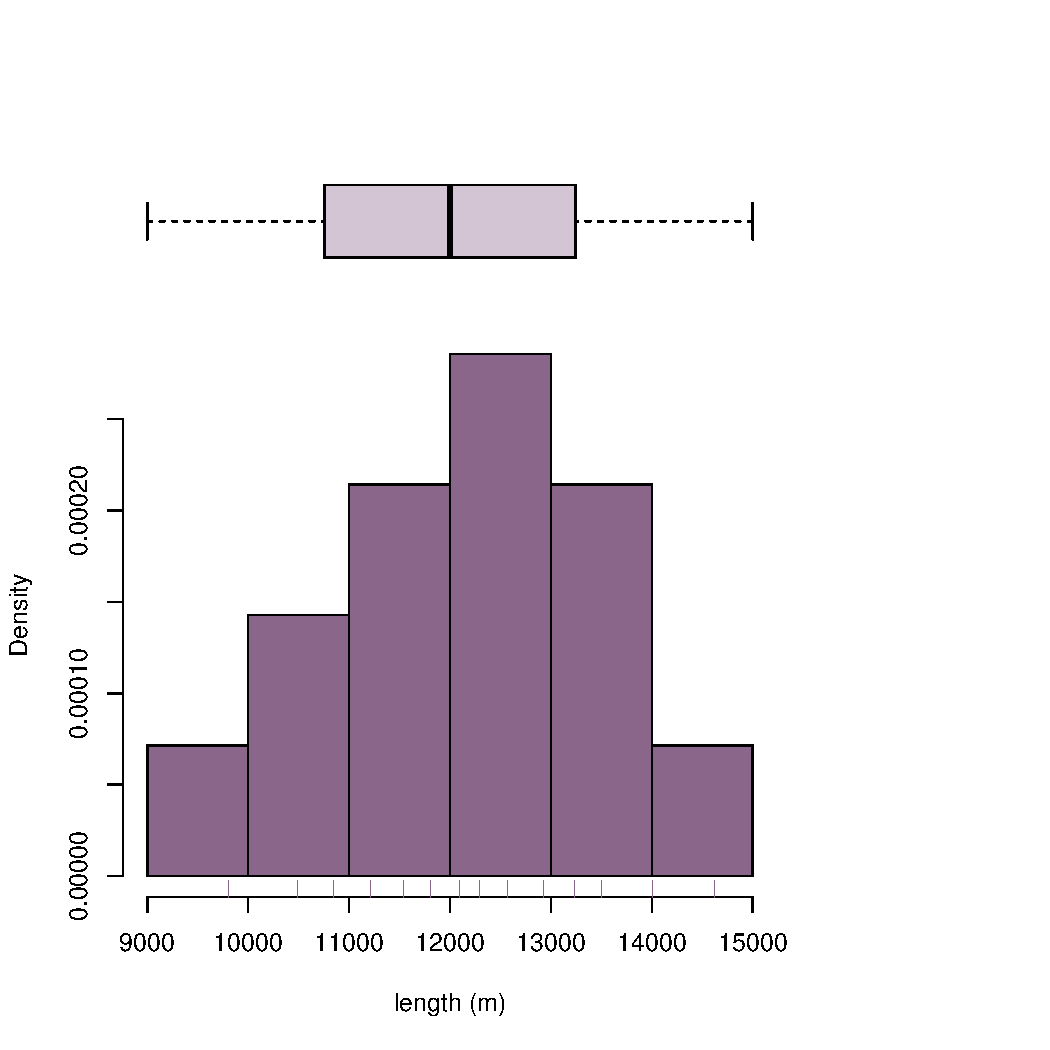
\includegraphics[width=7cm,height=7cm]{figure/BoxCoxhistplots3} 
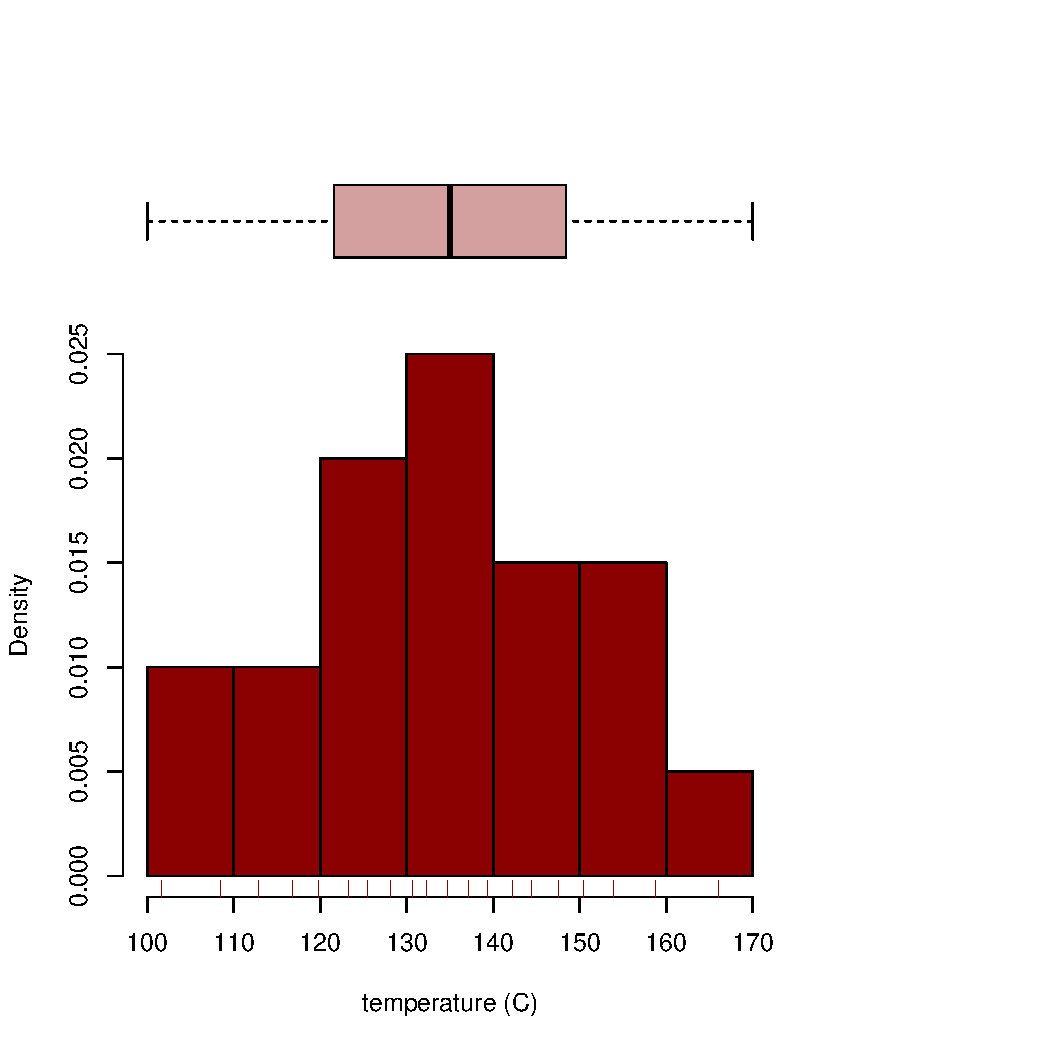
\includegraphics[width=7cm,height=7cm]{figure/BoxCoxhistplots4} \caption[Normalized parameter distributions using normal score transform]{Normalized parameter distributions using normal score transform\label{Fig:BoxCoxhistplots}}
\end{figure}


\end{knitrout}

\begin{knitrout}
\definecolor{shadecolor}{rgb}{0.969, 0.969, 0.969}\color{fgcolor}\begin{figure}[]

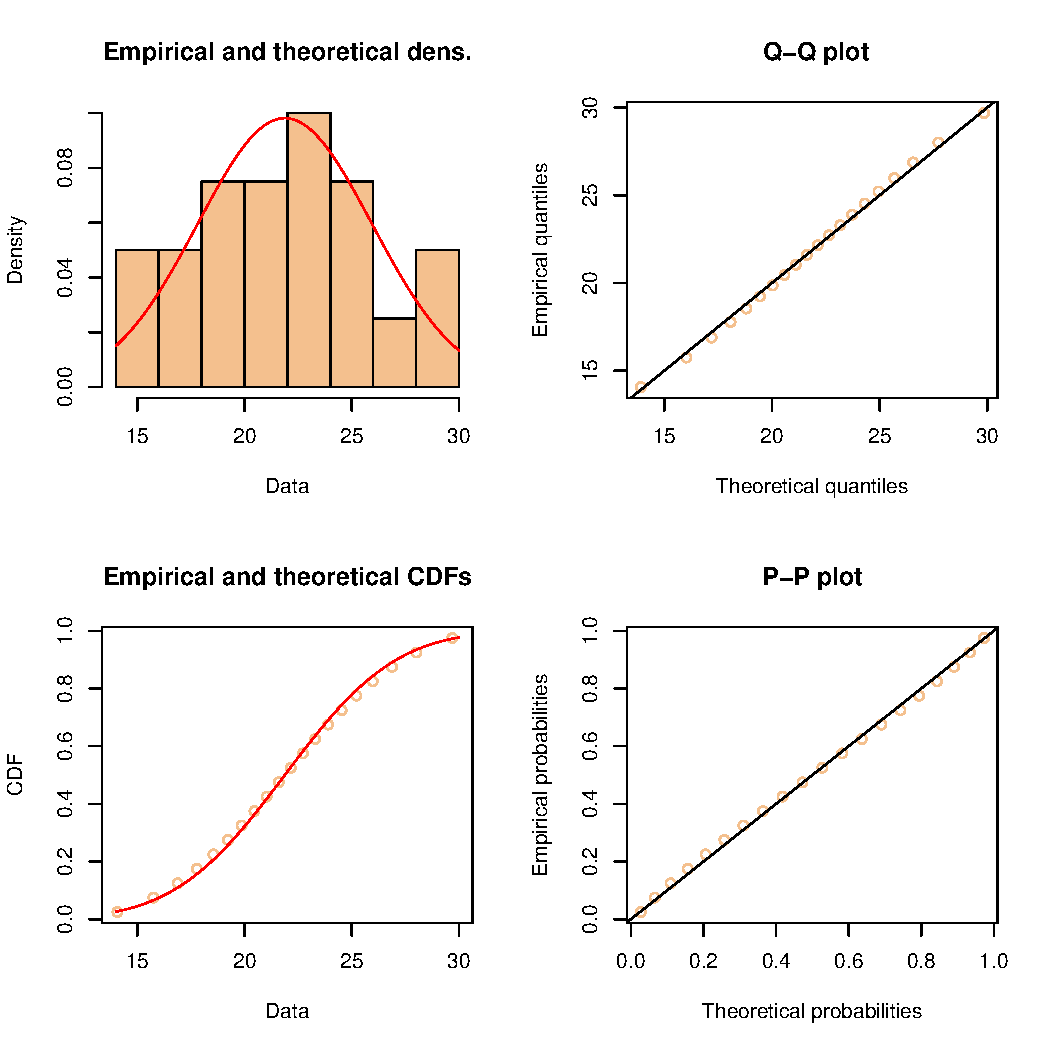
\includegraphics[width=\maxwidth]{figure/poro_norm_fit} \caption[Gaussian distribution fitted to the normalized porosity]{Gaussian distribution fitted to the normalized porosity. As expected, both Q-Q and the CDF plot indicate good fit.\label{Fig:poro_norm_fit}}
\end{figure}


\end{knitrout}


% latex table generated in R 3.1.1 by xtable 1.7-3 package
% Wed Aug 06 14:17:31 2014
\begin{table}[ht]
\centering
\begin{tabular}{rrrrr}
  \hline
 & porosity & tickness.m & length.m & temperature.C \\ 
  \hline
mean & 21.88 & 103.42 & 12198.87 & 133.72 \\ 
  sd & 4.07 & 35.18 & 1317.48 & 16.73 \\ 
   \hline
\end{tabular}
\caption{{Summary of the gaussian fit to the porosity, thickness, length and temperature}} 
\label{Tab:poro_etc_fit}
\end{table}



\pagebreak


%-----------------------------------------------
%                 Earth thermal gradient
%-----------------------------------------------
\section{Geothermal gradient}
Geothermal gradient of the earth appears in the buoyancy dimensionless number. The mean geothermal graident varies from less than 15 C/km to more than 50 C/km on a regional basis. Depending on the lithology, this variation can be up to a factor of 5 or more in a single well \citep{tester2006future}. \citet{Gray2010} has studied the geothermal gradient for the wells on the Guyana dome and concluded that sediments shallower than 3900 m have an average thermal gradient of 23 C/km. They suggest a geothermal gradient of 28.9 C/km from the depth of 3900 to 5000 m based on the well temperature data and contributes it to geopressured layers formed by rapid sedimentation. Average geothermal gradient is around 25 C/km in most of the world \citep{fridleifsson2008possible} and it turned out to be very close to the averaged value for the whole sedimentary section estimated in this study.  We used depth and temperature data from the wells to estimate the geothermal gradient (e.i. regression coefficient, Figure \ref{Fig:geothermal_gradient}). 

To establish a confidence interval for the calculated geothermal gradient without assuming any underlying theoretical distribution, a repeated random sampling with replacemnt (bootstrapping) is performed (Figure \ref{Fig:bootstrap_plot}, \citet{white_note}).  

\begin{knitrout}
\definecolor{shadecolor}{rgb}{0.969, 0.969, 0.969}\color{fgcolor}\begin{figure}[]

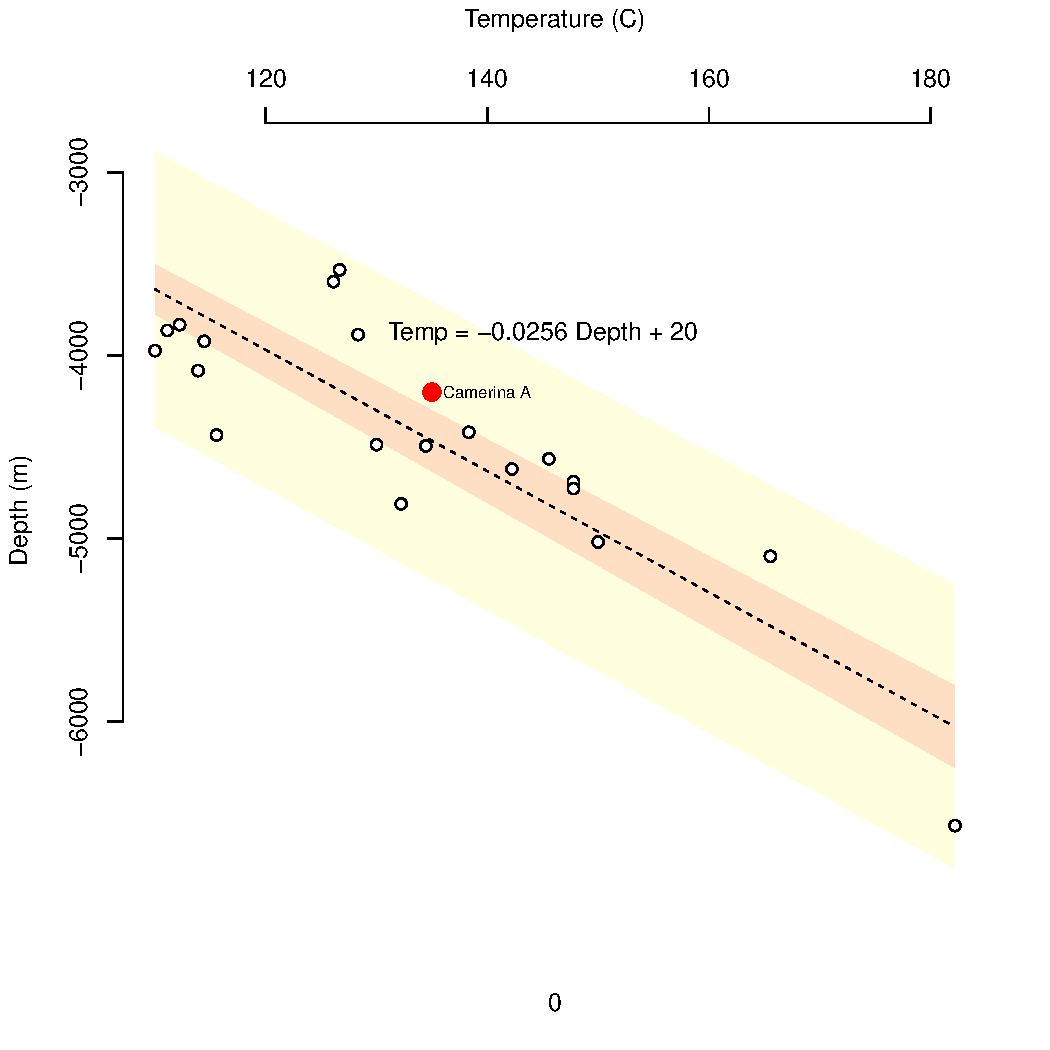
\includegraphics[width=\maxwidth]{figure/geothermal_gradient} \caption[The dark tan region shows 95\% confidence interval band around the predicted mean for the temperature of the geothermal reservoirs in Louisiana at each depth]{The dark tan region shows 95\% confidence interval band around the predicted mean for the temperature of the geothermal reservoirs in Louisiana at each depth. Average geothermal gradient is around 25 \degree C/km in most of the world \citep{fridleifsson2008possible} and the average value estimated here turned out to be very close. The light tan shows the 95\% confidence interval for the mean of any random sample. Camerina A reservoir is used to test the model and the model seems to be acceptable. Source code is modified from \citet{white_note}.\label{Fig:geothermal_gradient}}
\end{figure}


\end{knitrout}


%-------------------------------------------------------
%                Bootstraping thermal gradient



\begin{knitrout}
\definecolor{shadecolor}{rgb}{0.969, 0.969, 0.969}\color{fgcolor}\begin{figure}[]

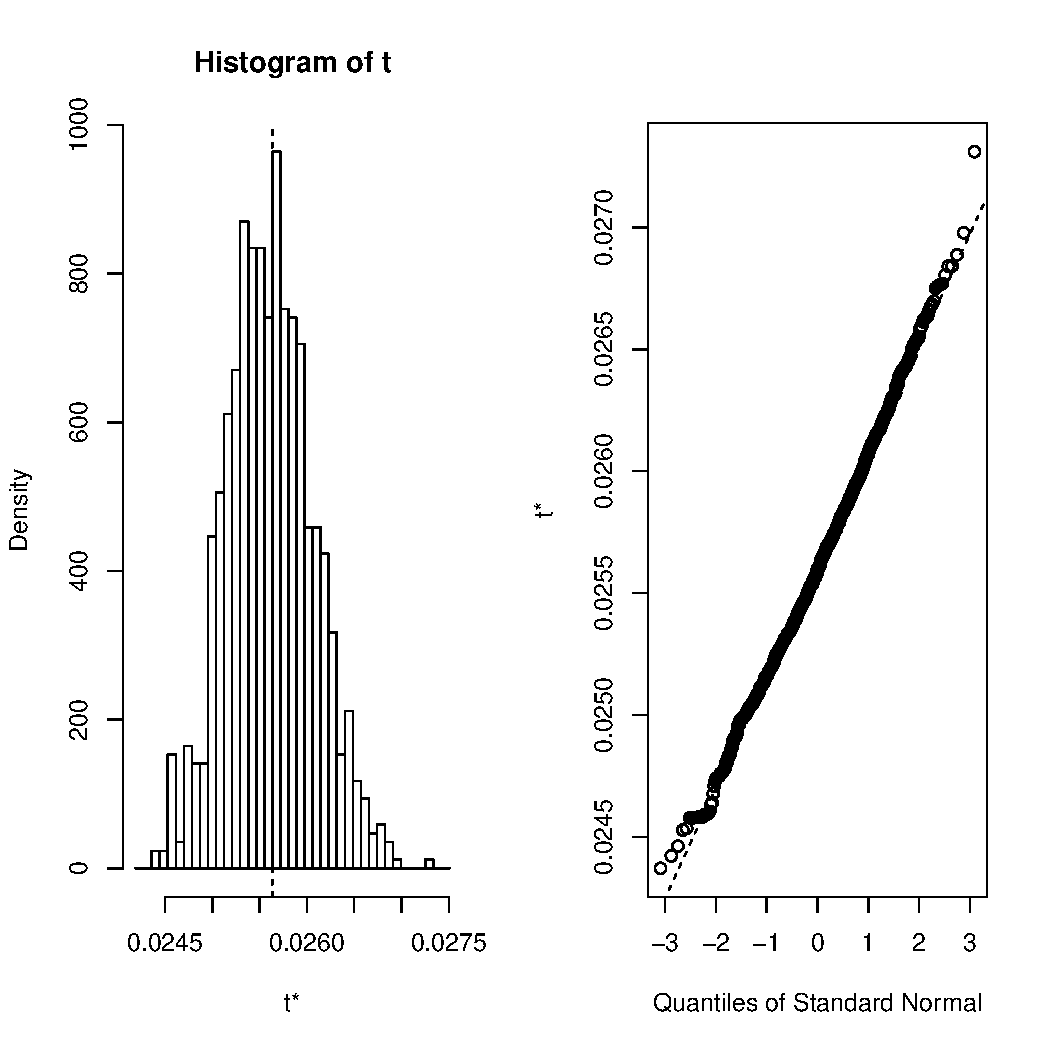
\includegraphics[width=\maxwidth]{figure/bootstrap_plot} \caption[Bootstrapped geothermal gradient of the earth for hot saline aquifers of the Louisiana]{Bootstrapped geothermal gradient of the earth for hot saline aquifers of the Louisiana. As expected, the value calculated for the mode is the same as the slope of the previous figure. The average geothermal gradient changes in the range 0. 024-0.027.\label{Fig:bootstrap_plot}}
\end{figure}


\end{knitrout}




%-----------------------------------------------
%               Dip Angle
%-----------------------------------------------
\section{Reservoir dip angle}
According to \citet{Gray2010}, the range of the dip angle for Camerina A reservoir is from 1.2\degree to 28\degree. Calculating the reservoir dip angle by investigating the gradient of the structural maps is challenging. Further, we are interested in the avereage reservoir dip angle and not the local dip angle. Exploratory data analysis is used to calculate this average dip angle \citep{diggle2007model}. It is done by recognizing that the temperature of the Louisiana's geopressured-geothermal reservoirs would remain lower than $T_{max}$ and by using reservoir's temperature gradient, average temperature and its length (Figure \ref{Fig:Schematic}). Since no 'a priori' exists about where the average reservoir temperature or bottomhole temperature attributes to, we assume that the data are sampled uniformly along the reservoir assigning teh average reessvoir temperature to (L/2,H/2). Available data can be used to calculate this $T_{max}$ using Eq. \ref{Fig:Schematic}.


\begin{figure}
\centering
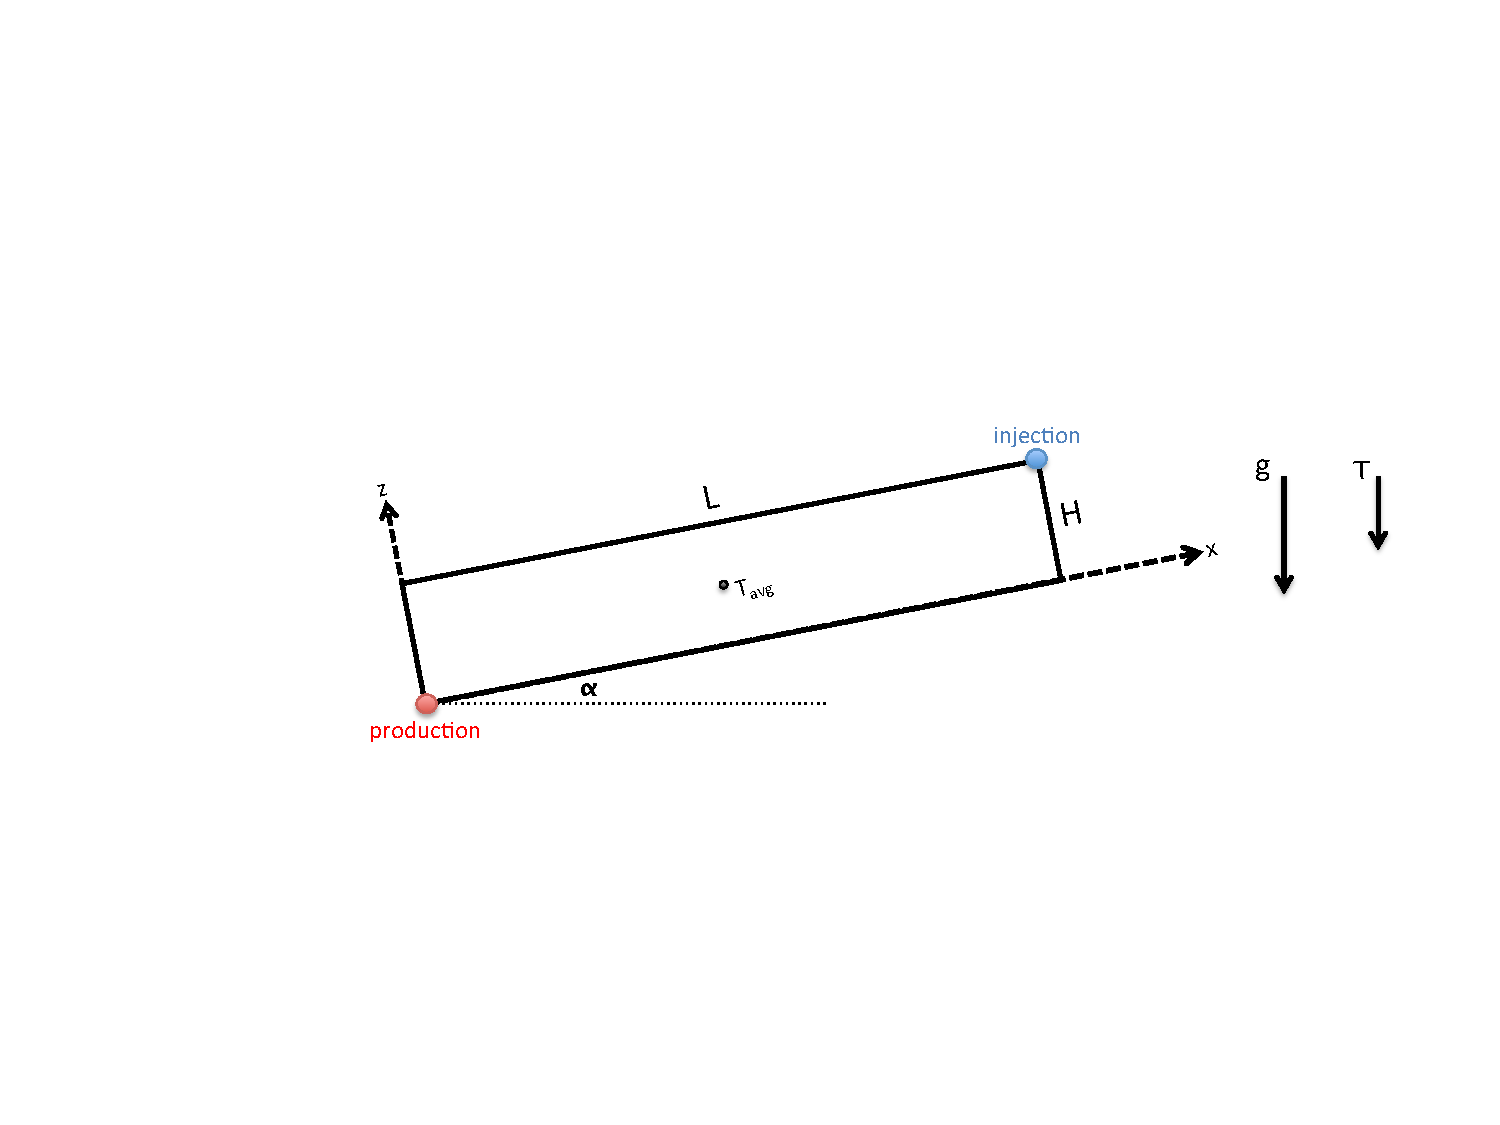
\includegraphics[width=0.75\linewidth]{./figure/schematic}
\caption{Regular design.} 
\label{Fig:Schematic}
\end{figure}


%\begin{equation}
%\tau \frac{L}{2} \sin \alpha + T_{avg} = T_{max}
%\end{equation}

\begin{equation}
\label{Eq:DipModel}
\alpha = \sin^{-1} \left(\frac{2(T_{max}-T_{avg})}{\tau L}\right)
\end{equation}

in which:

\begin{eqnarray}
\tau \sim \mathcal{N}(\mu_\tau,\sigma^2_\tau) \\
T_{avg} \sim \mathcal{N}(\mu_T,\sigma^2_T) \\
L \sim \mathcal{N}(\mu_L,\sigma^2_L) \\
T_{max}=?
\end{eqnarray}

Knowing that the dip angle of Eq. \ref{Eq:DipModel} can not be more than 90 degrees, we can find $T_{max}$ with the probability of $0.99*0.99=0.9801$ by constraining the fraction in Eq. \ref{Eq:DipModel} to its maximum (i.e. one) which means:

\begin{equation}
\frac{2(T_{max}-T_{avg})}{\tau L} \leq 1 
\end{equation}
\begin{equation}
T_{max} \leq T_{avg}+\frac{\tau L}{2} 
\end{equation}
\begin{equation}
T_{max} = ({\mu_T-3\sigma_T})+\frac{(\mu_{\tau}-3\sigma_{\tau})(\mu_{L}-3\sigma_L)}{2}
\label{Eq:TmaxSolution}
\end{equation}



Once $T_{max}$  is found to be ca. 183 $^\circ C$, we can solve Eq. \ref{Eq:DipModel} using a sampling method \citep{kroese2011handbook}. We used Hammersley Sequence Sampling to sample average temperature, geothermal gradient and reservoir's length for finding the dip angle of the layers (Figure \ref{Fig:dip_angle}). The median of the dip angle is ca. 15\degree and . If we exclude the outliers, it is unlikely to have a reservoir with the dip angle of more than ca. 60\degree. The lower quartile is ca. 2.5\degree and the upper quartile is ca. 25\degree.



\begin{knitrout}
\definecolor{shadecolor}{rgb}{0.969, 0.969, 0.969}\color{fgcolor}\begin{figure}[]


{\centering 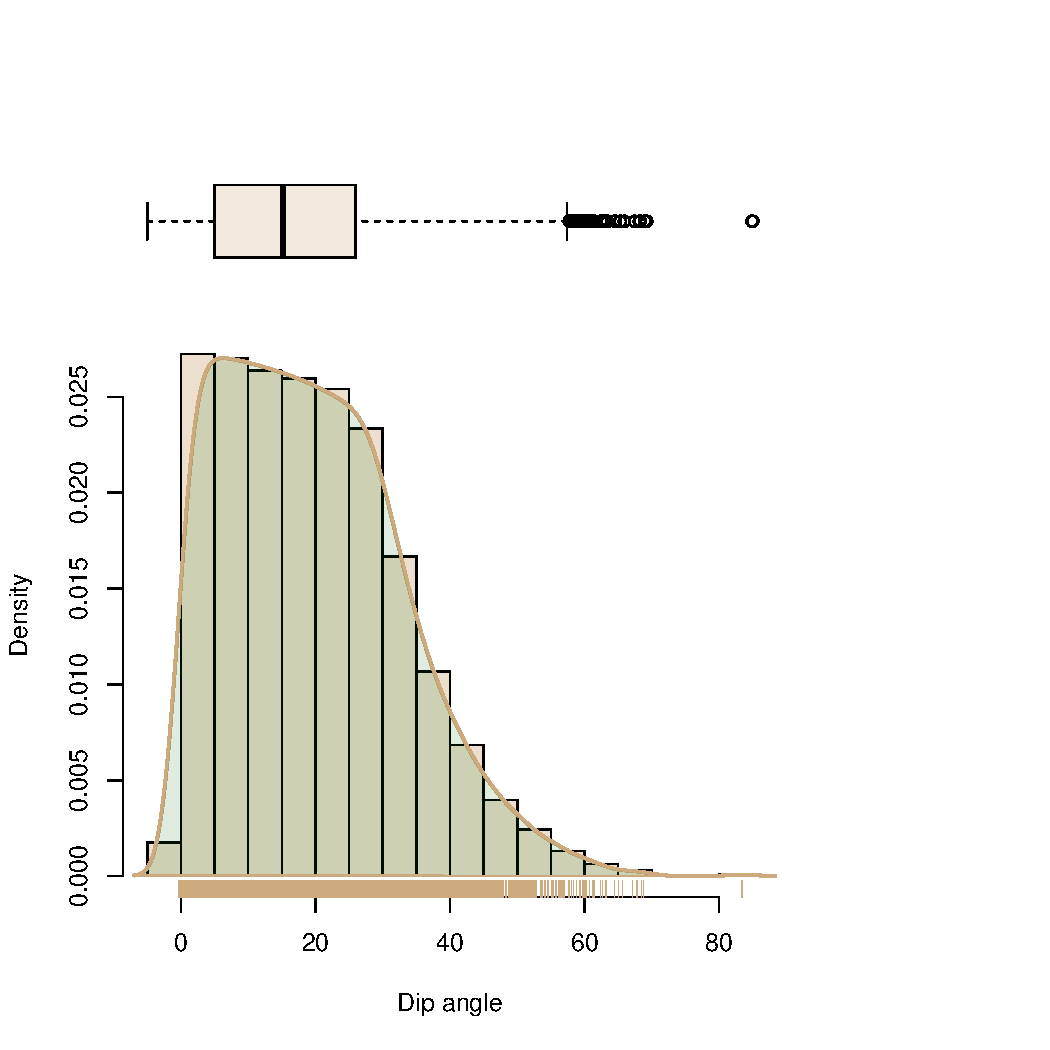
\includegraphics[width=10cm,height=10cm]{figure/dip_angle} 

}

\caption[Distribution of the Gulf Coast geothermal reservoir's dip angle]{Distribution of the Gulf Coast geothermal reservoir's dip angle. The median of the dip angle is ca. 15\degree and . If we exclude the outliers, it is unlikely to have a reservoir with the dip angle of more than ca. 60\degree. The lower quartile is ca. 2.5\degree and the upper quartile is ca. 25\degree.\label{Fig:dip_angle}}
\end{figure}


\end{knitrout}


%-----------------------------------------------
%                Injection temperature
%-----------------------------------------------
\section{Injection temperature}
Injection temperature reduces the temperature of the reservoir. In binary power plants, the discharge temperature varies in a large range 25-90 \degree C \citep{tester2006future}. Average annual surface temperature for the Louisiana is ca. 20 \degree C (www.ncdc.noaa.gov); so it is more likely that the injection temperature further reduces to this temperature. Though the range of injection temperature is known, no 'a priori' knowledge of the distribution form is available. When there is a most likely value within a range but no 'a priori' knowledge, a triangular distribution is appropriate (Figure \ref{Fig:injectionTemp}, \citet{jensen2000statistics}). The triangle is defined using the range 20-90 \degree C and it's most likely value as 20 \degree C.

\begin{knitrout}
\definecolor{shadecolor}{rgb}{0.969, 0.969, 0.969}\color{fgcolor}\begin{figure}[]


{\centering 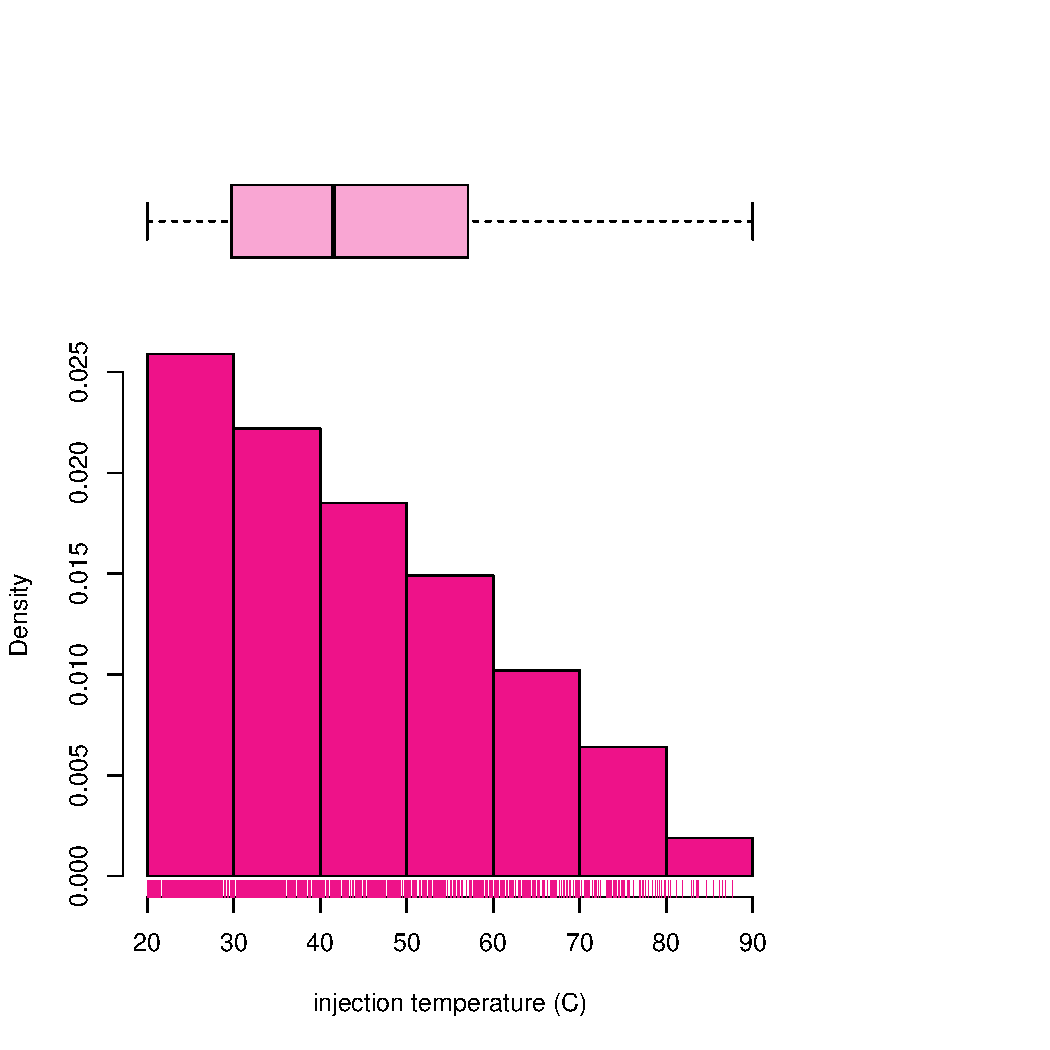
\includegraphics[width=7cm,height=7cm]{figure/injectionTemp} 

}

\caption[injection temperature for binary power plants]{injection temperature for binary power plants\label{Fig:injectionTemp}}
\end{figure}


\end{knitrout}

For downhole heat exchangers, the injection temperature is a function of  its production section's length, its middle length, its injection section's length, input temperature and other factors such as working fluid, casing and tubing diameter, etc (Fig. \ref{Fig:DHEscheme}). A DHE with working fluid injected through the tubing and brine passing the casing is known as WFT (working fluid through tubing) which has higher efficiency compared with other designs. DHE's total length varies between ca. 150 and 300 m which makes the injection temperature varying from ca. 120 down to 40 C respectively for an input temperature of ca. 150 C, and flow rate of ca. 400 m\textsuperscript{3}.day\textsuperscript{-1}, assuming engineering assumptions for other parameters \citep{feng2012numerical}. A uniform distribution can be used for DHE's injection temperature because no 'a priori' knowledge is available. 

\begin{figure}
\centering
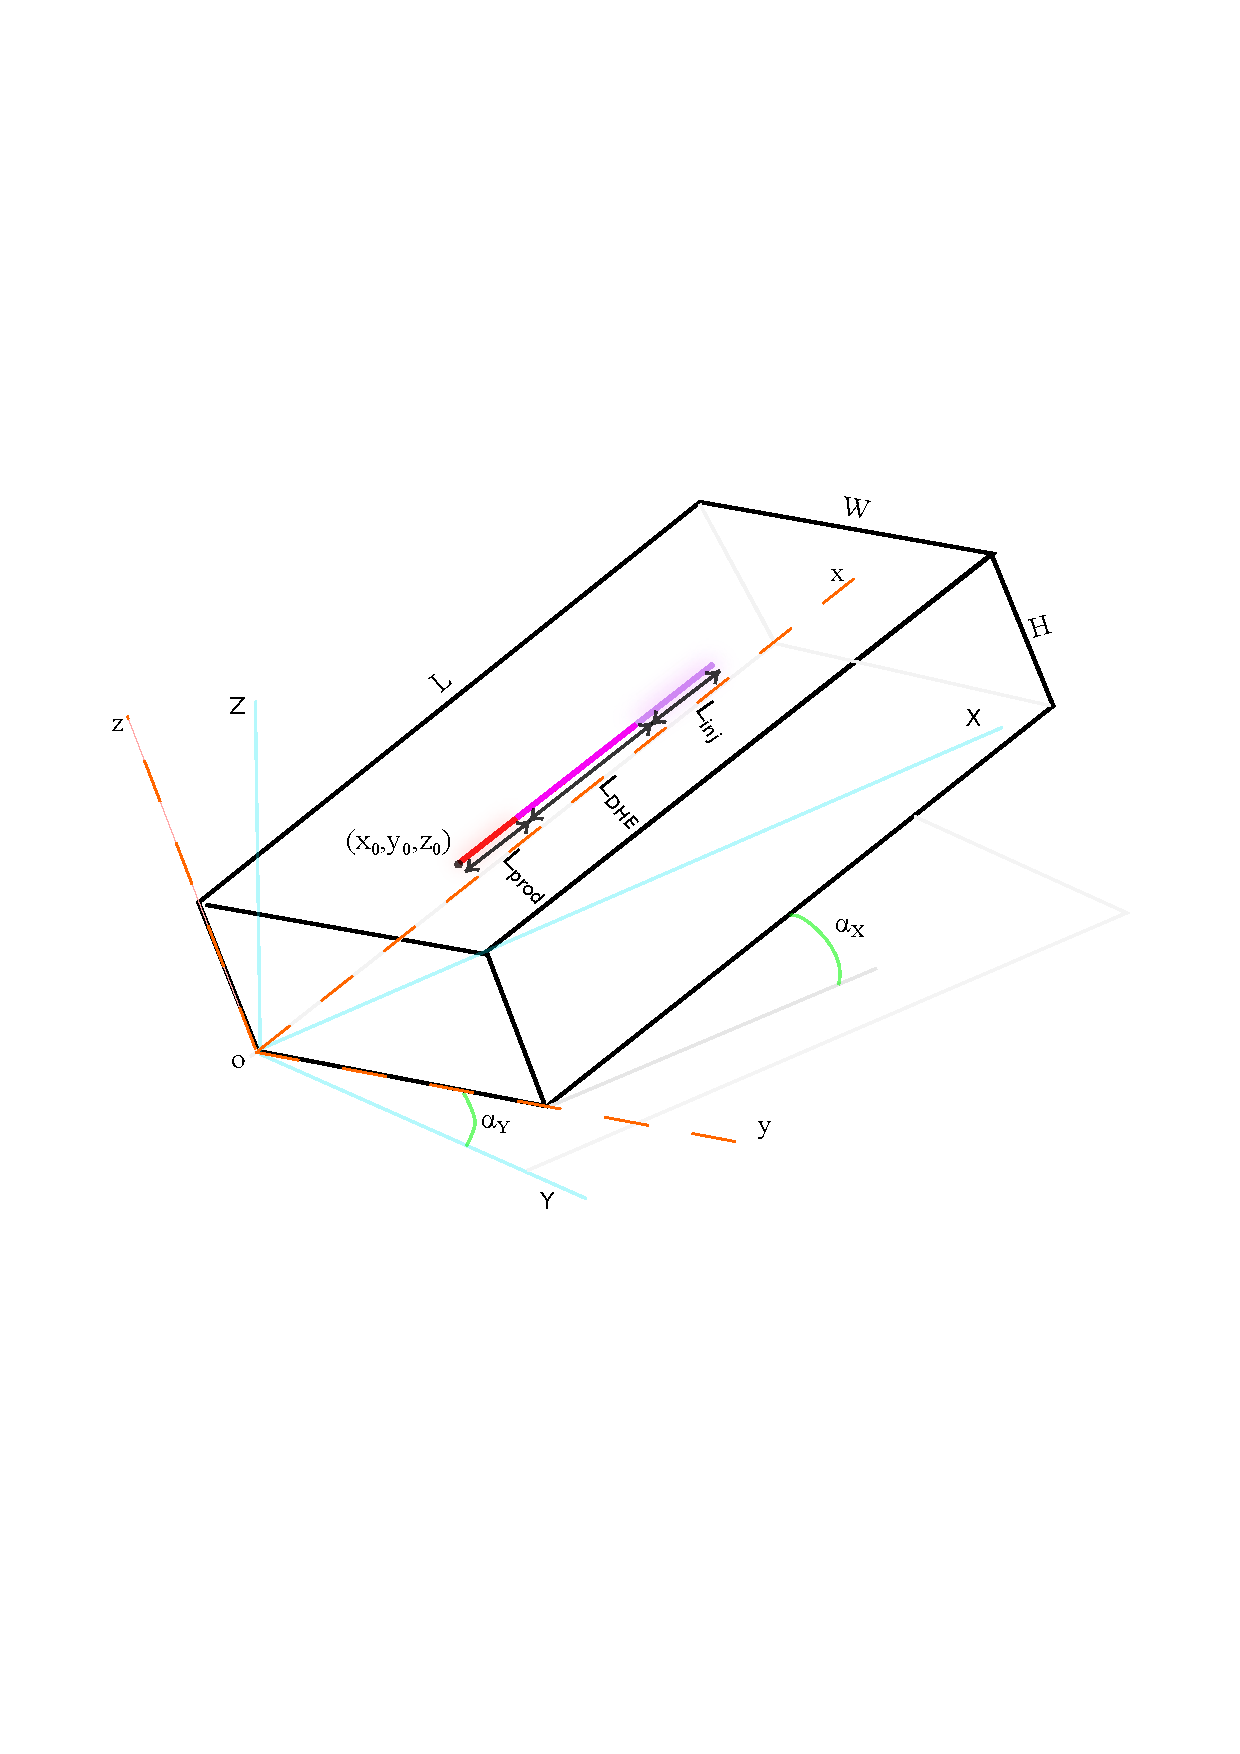
\includegraphics[width=0.75\linewidth]{./figure/DHE}
\caption{DHE scheme that is being used for dimensional analysis.} 
\label{Fig:DHEscheme}
\end{figure}
 


%-----------------------------------------------
%                   Flow Rate
%----------------------------------------------
\section{Flow Rate}
Flow rate is also a very important parameter and rate of power generation directly depends on it. It seems the reported flow rate for the well tests are restricted by TPR curves because the reservoir models can sustain higher rates. In fact Gulf Coast geopressured aquifers came to attention for their geohydraulic potential rather than their geothermal energy \citep{Hawkins1977}. \citet{McMullan1984} realizing that maximizing flow-rate maximizes NPV in geopressured geothermal reservoirs, showed that the effect of tubing size and skin overwhelms other effects such as well location with respect to aquifers. Their study indicates that these reservoirs can sustain higher than 6350 m\textsuperscript{3}.day\textsuperscript{-1} (40000 bbl.day\textsuperscript{-1}) and up to 17500 m\textsuperscript{3}.day\textsuperscript{-1} (110000 bbl.day\textsuperscript{-1}) for maximum of 5 years. The well test data shows a flow rate of ca. 250 to 4250 m\textsuperscript{3}.day\textsuperscript{-1} (Figure \ref{Fig:flowrate}). A unifrom distribution can be used for flow rate because there is no priori knowledge of the distribution and based on the current data, we can certainly say that the variable cannot take values outside well test recorded range. 

\begin{knitrout}
\definecolor{shadecolor}{rgb}{0.969, 0.969, 0.969}\color{fgcolor}\begin{figure}[]


{\centering 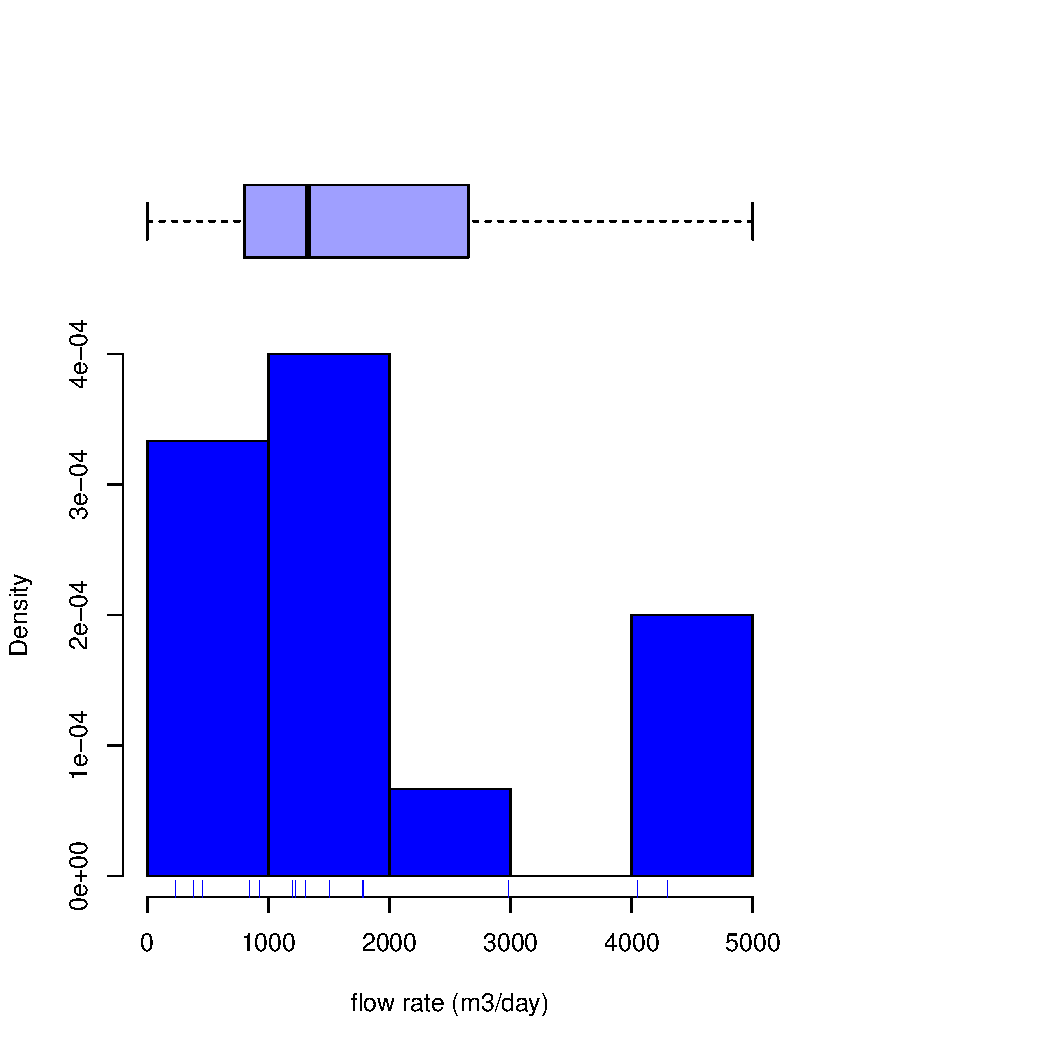
\includegraphics[width=7cm,height=7cm]{figure/flowrate} 

}

\caption[Well test data for flow rate]{Well test data for flow rate\label{Fig:flowrate}}
\end{figure}


\end{knitrout}

Previous DHE designs have single point fluid inlet and single point or a length fluid for outletting the fluid and are insulated from the reservoir \citep{feng2012numerical}. However the new designs are evolving into having a length for production and a length for injection. Also, the DHE's middle (main) length is not isolated from the reservoir (Ildar, personal communication) and its flow rate is lower than conventional heat exchangers (ca. 450 m\textsuperscript{3}.day\textsuperscript{-1} or 5.25 kg.s\textsuperscript{-1}) \citep{feng2012numerical} which seemingly cannot be increased due to DHE's limitations such as sand production, pump capacity, etc. (Ildar, personal communication). 




%\section*{References}
\bibliographystyle{elsarticle-harv}
\bibliography{./sections/Bibliography}



\end{document}
